\documentclass[12pt]{article}
\usepackage[usenames]{color} %used for font color
\usepackage{amsmath, amssymb, amsthm}
\usepackage{wasysym}
\usepackage[utf8]{inputenc} %useful to type directly diacritic characters
\usepackage{graphicx}
\usepackage{caption}
\usepackage{subcaption}
\usepackage [english]{babel}
\usepackage [autostyle, english = american]{csquotes}
\MakeOuterQuote{"}
\graphicspath{ {./} }
\newcommand{\Z}{\mathbb{Z}}
\newcommand{\N}{\mathbb{N}}
\newcommand{\R}{\mathbb{R}}
\newcommand{\Q}{\mathbb{Q}}
\newcommand{\prob}{\mathbb{P}}
\newcommand{\degrees}{^{\circ}}


\author{Tianshuang (Ethan) Qiu}
\begin{document}
\title{Math 74, Week 5}
\maketitle


\section{Mon Lec, 2a}
Let the statement: "There is at most one parallel line to a given line $l$ through a given point $P$." be statement A;
\newline
"If a line intersects one of two parallel lines, both of which are coplanar with the original line, then it also intersects the other." be statement B.
\newline
\begin{figure}[h]
    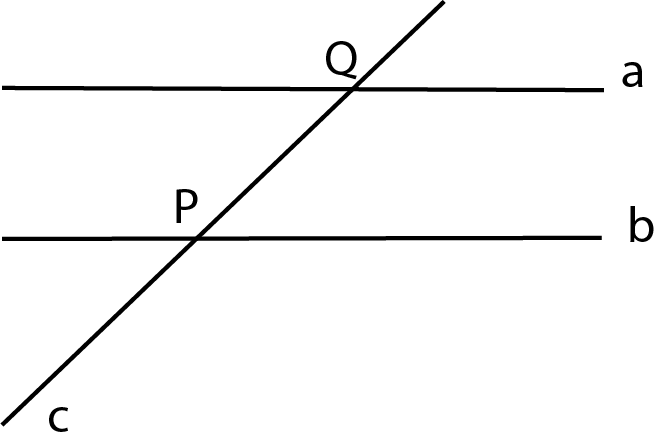
\includegraphics[width = 100mm]{GRAPH1.png}
\end{figure}
\newline
We first prove that $A \implies B$. Let $a \parallel b$, and $c$ intersects $a$ at point $Q$. Assume that statement $B$ is false so $c$ does not intersect $b$. Since it does not intersect and $b$ and $c$ are coplanar, we have $b \parallel c$. $a \parallel b$, and $a, c$ interesect at $Q$. However by $A$ we know that there can be at most one line parallel to $b$ at point $Q$. \lightning. Our assumption is incorrect, $A \implies B$
\newline
Then we show that $B \implies A$. Let $a \parallel b$, and $c$ intersects $b$ at point $P$. Assume that $A$ is incorrect, so we construct $a'$ to also be parallel to $b$. We know that $b$ must intersect $a$ by $B$. We name this point $P$. Then since we have assumed that $a \parallel a'$, our line must also intersect $a'$ at $P$. Consider $\angle SPT, \angle RQT$, and they must be equal because they $a \parallel b$, and corresponding angles are equal when the two lines are parallel. By the same logic we have $\angle SPT = \angle R'QT$.
\newline
Using the transitive property we can get $\angle RQT = \angle R'QT$. However this cannot be true because if the two angles are equal, $a, a'$ overlap and they become the same line. \lightning
\newline
Our assumption is incrroect and $B \implies A$. Therefore $A \iff B$. Q.E.D.

\section{Mon Lec, 3a}
\begin{figure}[h]
    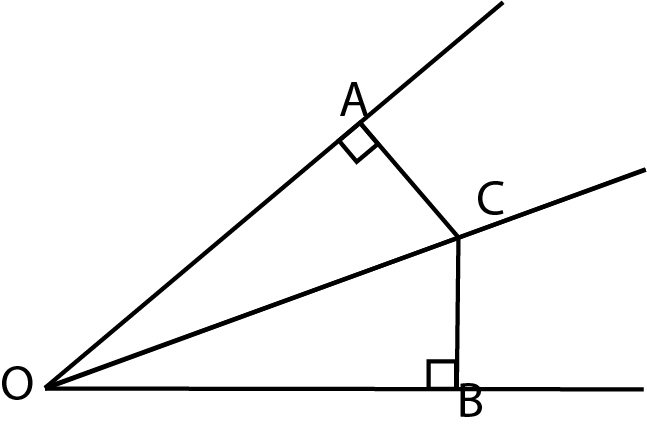
\includegraphics[width = 100mm]{GRAPH2.png}
\end{figure}
\subsection{Bisector $\implies$ equal distance from legs}
Let $OC$ bisect $\angle AOB$, choose $A, B$ such that $CA \perp OA, CB \perp OB$
\newline
Consider $\triangle AOC, BOC$, since $CA \perp OA, CB \perp OB$, we can write the following using the inner sum of triangles:
$$\angle ACO + \angle COA + 90 \degrees = 190 \degrees$$
$$\angle BCO + \angle COB + 90 \degrees = 190 \degrees$$
Since $OC$ bisect $\angle AOB$, we have $\angle COA = \angle COB$, so $\angle ACO = \angle BCO$. Finally, since $\triangle AOC, BOC$ share $OC$, we have $\triangle AOC \cong \triangle BOC$ (ASA congruency). Therefore $CA = CB$. Q.E.D.

\subsection{Equal distance from legs $\implies$ angle bisection}
Let $OC$ be a ray from $O$, choose point C and draw $CA \perp OA, CB \perp OB$. $AC = BC$
\newline
Consider $\triangle AOC, BOC$, since $CA \perp OA, CB \perp OB$, they are both right triangles. Using $AC = BC$, we have $\triangle AOC \cong \triangle BOC$ (HL right triangle congruency). Therefore $\angle COA = \angle COB$.
Q.E.D.
\newpage


\section{Mon Dis, 1b (second bullet)}
$$\prod^{n}_{1}=(1-\frac{1}{n^2})$$
We examine $1-1/k^2$ and factor it into $\frac{k^2-1}{k^2} = \frac{(k+1)(k-1)}{k^2}$. Since k is incrementing by 1 in our series, we can cancel the majority of terms out since it is telescoping. We can expand our series into
$$\frac{1\times 3}{2^2} \times \frac{2 \times 4}{3^2} \times ...\times \frac{(n-1)(n+1)}{n^2}$$
$$= \frac{1}{2} \times \frac{n+1}{n} = \frac{n+1}{2n}$$

\section{Mon Dis, 1d}
(Assuming that )
\subsection{$4^n + 15n -1$}
The largest common divisor for these expressions is $1$.

\subsection{$n^3 - n$}
The largest common divisor for these expressions is $6$.

\subsection{$2^{n+2} + 7n$}
The largest common divisor for these expressions is $5$.
\newpage


\section{Wed Lec, 3a}
Base case: $n = 1, 1 = 1^2$. Base case holds.
\newline
Inductive hypothesis: assume that for some $n \geq 1$, $1+ 3 + 5 + ... + (2n-1) = n^2$.
\newline
Inductive proof: consider $n+1$, $1+ 3 + 5 + ... + (2n-1) + (2n+1)$, using our inductive hypothesis, we can susbsitute everything but the last term: $n^2 + 2n + 1 = (n+1)^2$
\newline
Thus we have proven the inductive step. Q.E.D.

\section{Wed Lec, 3c}
Base case: $n = 1, 1/(4 \times 1^2 - 1) = 1/3 = 1/(2 \times 1 + 1)$. Base case holds.
\newline
Inductive hypothesis: assume that for some $n \geq 1$, $\frac{1}{4 \times 1^2 - 1} + \frac{1}{4 \times 2^2 - 1} + ... + \frac{1}{4 \times n^2 - 1} = \frac{n}{2n+1}$.
\newline
Inductive proof: consider $n+1$, $$\frac{1}{4 \times 1^2 - 1} + \frac{1}{4 \times 2^2 - 1} + ... + \frac{1}{4 \times n^2 - 1} + \frac{1}{4 \times (n+1)^2 - 1}$$
Using our inductive hypothesis, we can susbsitute everything but the last term: $$\frac{n}{2n+1} + \frac{1}{4(n+1)^2 - 1} = \frac{n (4(n+1)^2-1)}{(2n+1)(4(n+1)^2-1)} + \frac{2n+1}{(2n+1)(4(n+1)^2 - 1)}$$
$$=\frac{n(4n^2+3+8n) + 2n +1}{(2n+1)(4n^2+3+8n)} = \frac{4n^3+3n+8n^2+2n+1}{8n^3+6n+16n^2+4n^2+3+8n}=\frac{4n^3+8n^2+5n+1}{8n^3+20n^2+14n+3}$$
We apply long division by $2n+3$ to the denominator.
$$\frac{8n^3+20n^2+14n+3}{2n+3} = 4n^2 + 4n + 1$$
Now we apply long division by $n+1$ to the numerator.
$$\frac{4n^3+8n^2+5n+1}{n+1} =  4n^2 + 4n + 1$$
Therefore we can factor the expression into
$$\frac{(n+1)(4n^2 + 4n + 1)}{(2n+3)(4n^2 + 4n + 1)} = \frac{n+1}{2n+3}$$
\newline
Thus we have proven the inductive step. Q.E.D.

\section{Wed Lec, 6b}
We claim that we can divide a single square into all $n \in \N, n \geq 6$ squares.
\newline
First we define a process of "opening a window": by connecting midpoints of sides that are across each other, we draw a cross on a square, dividing it into 4 smaller squares. The total gain of this process is $4-1=3$ squares.
\newline
We split the cases into the following: $n = 3k, n = 3k+1, n = 3k+2 (k \geq 2)$, and we will prove by induction each case.
\newline
Base cases: $n = 6, 7, 8$, we can divide it up like the following:
\newline
\begin{figure}[h]
     \centering
     \begin{subfigure}[b]{0.3\textwidth}
         \centering
         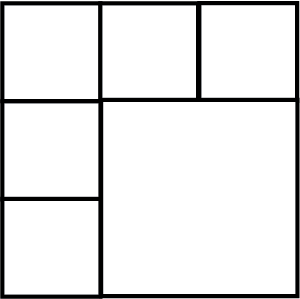
\includegraphics[width=\textwidth]{GRAPH5}
         \caption{$n=6$}
     \end{subfigure}
     \hfill
     \begin{subfigure}[b]{0.3\textwidth}
         \centering
         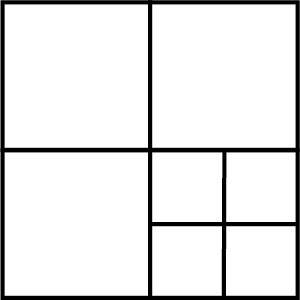
\includegraphics[width=\textwidth]{GRAPH4}
         \caption{$n=7$}
     \end{subfigure}
     \hfill
     \begin{subfigure}[b]{0.3\textwidth}
         \centering
         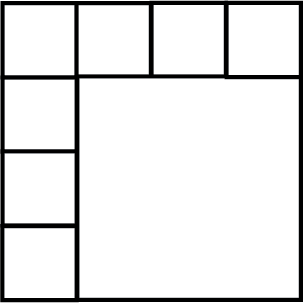
\includegraphics[width=\textwidth]{GRAPH3}
         \caption{$n=8$}
         \label{fig:five over x}
     \end{subfigure}
\end{figure}
\newline
Inductive case: Assume that for some $k \geq 2$, we can divide a square into $3k, 3k+1, 3k+2$ smaller squares, then in order to get $3(k+1)$ squares, we can simply "open a window" in any of the $3k$ sub squares. This yields a total of $3k+3 = 3(k+1)$ squares.
\newline
We can prove the cases for $3(k+1)+1, 3(k+1)+2$ by also "opening a window" using a subsquare in squares that has been divided into $3k+1$ and $3k+2$ parts, yielding $3k+4$ and $3k+5$ squares.
\newline
Thus we have proven the inductive case. Q.E.D.
\newpage


\section{Wed Dis, 3a}
Base case: $n=1$, $1^3 = (1\times2/2)^2 = 1$, base case holds.
\newline
Inductive case: Assume that $$1^3 + 2^3 + ... + n^3 = (\frac{n(n+1)}{2})^2$$
for some $n \geq 1$, consider
$1^3 + 2^3 + ... + n^3 + (n+1)^3$, we can apply our inductive hypothesis to get
$$ = (\frac{n(n+1)}{2})^2 + (n+1)^3 = \frac{n^2(n+1)^2}{4} + (n+1)^3 = \frac{n^2(n+1)^2+4(n+1)^3}{4}$$
$$= \frac{(n+1)^2(n^2+4(n+1))}{4} = \frac{(n+1)^2(n^2+4n+4)}{4} = (\frac{(n+1)^2(n+2)^2}{2^2})$$
The expression above is exactly what we would expect if we subsitute $(n+1)$ for $n$ in $(\frac{n(n+1)}{2})^2$. Therefore we have proven the inductive case. Q.E.D.

\section{Wed Dis, 4a}
Base case: $n = 0, 1 = (x-1)/(x-1) = 1$ since $x \neq 1$. Base case holds.
\newline
Inductive case: Assume that the statement is true for some $n \geq 0$. Consider $n+1$, we have: $1 + x + x^2 + ... + x^n + x^{n+1}$. Now we apply our inductive hypothesis:
$$= \frac{x^{n+1}-1}{x-1} + x^{n+1} = \frac{x^{n+1}-1+x^{n+1}(x-1)}{x-1} = \frac{x^{n+1}-1+x^{n+2}-x^{n+1}}{x-1} = \frac{x^{n+2}-1}{x-1}$$
The expression above is exactly what we would expect if we subsitute $(n+1)$ for $n$ in $\frac{x^{n+1}-1}{x-1}$. Thus we have proven the inductive case. Q.E.D.
\newpage


\section{Fri Lec, 2b}
$n! < n^n \forall n \geq 2$
\newline
Base case: $n=2, n!=2, n^n=4, n! < n^n$, base case holds.
\newline
Inductive case: assume that $n! < n^n$ for some $n \geq 2$, consider $(n+1)!, (n+1)^{n+1}$. By the definition of factorials we have $(n+1)! = (n+1)n! < (n+1)n^n$
\newline
Now, consider $(n+1)n^n, (n+1)^{n+1}$. Since the latter is $n+1$ multiplied by itself $n+1$ times, and the former only has $n+1$ once and $n$ n times, and since $n<n+1$, we have $(n+1)n^n < (n+1)^{n+1}$.
\newline
Now we can put it all together: $(n+1)! = (n+1)n! < (n+1)n^n < (n+1)^{n+1}$. Thus we have proven the inductive case. Q.E.D.

\section{Fri Lec, 3a}
Base case: $n = 0, n^3-n = 0, n \bmod 6 \equiv 0$ Base case holds.
\newline
Inductive case: Assume that $(n^3-n) \mid 6$ for some $n \geq 0$, consider $(n+1)^3-(n+1)$.
$$= n^3 + 3n^2 + 3n + 1 - n -1 = n^3+3n^2+2n = n(n^2+3n+2) = n(n+1)(n+2)$$
Integers that are divisible by 2 are spaced such that there is one every other, and those divisible by 3 are spaced such that there is one every third. Here we have a product of 3 consecutive integers, so there must be at least 1 integer between $n, n+1, n+2$ that is divisible by 2, and at least 1 that is divisible by 3. Since $6=2 \times 3$, we have $n(n+1)(n+2) \mid 6$.
\newline
We have proven the inductive case. Q.E.D.

\section{Fri Lec, 3b}
Base case: $n = 0, 2^2+7^0 = 5, 5 \bmod 5 \equiv 0$ Base case holds.
\newline
Inductive case: Assume that $2^{n+2}+7^n \mid 5$ for some $n \geq 0$, consider $2^{n+3}+7^{n+1}$.
\newline
We add then subtract $2^{n+2}\times 7$ from the latter, this does not change the value but will alow us to manipulate the terms:
$$7 \times 2^{n+2} - 7 \times 2^{n+2} + 2^{n+3}+7^{n+1} = 7(2^{n+2}+7^n)+2^{k+2}(2-7)$$
$$=7(2^{n+2}+7^n) - 5 \times 2^{k+2}$$
By the inductive hypothesis  $2^{n+2}+7^n \mid 5$, and since $-5 \mid 5$, both terms are divisible by 5, therefore the sum must also be divisible by 5.
\newline
We have proven the inductive case. Q.E.D.
\end{document}
